%% %% %% %%
%%
%% Parte A de la práctica
%%
%% %% %% %%

\documentclass[../procedimientos.tex]{subfiles}
\graphicspath{{\subfix{../../images/}}}

\begin{document}
\clearpage
\subsection{Parte A}
\subsubsection{Instrucciones}
Diseñe un circuito digital con compuertas que funcione de la siguiente forma:
Cuando $C$ se coloca en bajo se debe detectar y señalizar, con un diodo led de 
color verde, todos los números divisibles entre cuatro; el led rojo no debe 
encender. Si $C$ cambia a un nivel alto, entonces se debe detectar y 
señalizar, con un led de color rojo, todos los números divisibles entre tres 
y, además, con el led verde, los números divisibles por cinco. El conjunto de 
números es de 4 bits.
\begin{figure}[H]
  \centering
  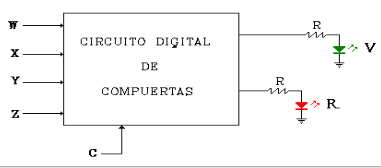
\includegraphics[width=0.5\textwidth]{a_instruction}
  \caption{Ejercicio A}
  \label{fig:a_inst}
\end{figure}

\subsubsection{Análisis}\label{subs:analisis_a}

\subsubsection{Implementación en Quartus}\label{subs:a_imp}

\end{document}

